% count/count.tex

\chapter{Counting}
\label{chp:Counting}

\QuickQuizChapter{chp:Counting}

Counting is perhaps the simplest and most natural for a computer to do.
However, counting efficiently and scalably on a large
shared-memory multiprocessor can be quite challenging.
Furthermore, the simplicity of the underlying concept of counting
allows us to consider concurrency issues without the distractions
of elaborate data structures or complex synchronization primitives.
Counting therefore provides an excellent introduction to
parallel programming.

This chapter covers a number of special cases for which there are simple,
fast, and scalable counting algorithms.
But first, let us find out how much you already know about concurrent
counting.

\QuickQuiz{}
	Why on earth should efficient and scalable counting be hard???
	After all, computers have special hardware for the sole purpose
	of doing counting,
	addition, subtraction, and lots more besides, don't they???
\QuickQuizAnswer{
	Because the straightforward counting algorithms, for example,
	atomic operations on a shared counter, are slow and scale
	badly, as will be seen in
	Section~\ref{sec:count:Why Isn't Concurrent Counting Trivial?}.
} \QuickQuizEnd

\QuickQuiz{}
	Suppose that you need to collect statistics on the number
	of networking packets (or total number of bytes) transmitted
	and/or received.
	Packets might be transmitted or received by any CPU on
	the system.
	Suppose further that this large machine is capable of
	handling a million packets per second, and that there
	is a systems-monitoring package that reads out the count
	every five seconds.
	How would you implement this statistical counter?
\QuickQuizAnswer{
	Hint: the act of updating the counter must be blazingly
	fast, but because the counter is read out only about once
	in five million updates, the act of reading out the counter can be
	quite slow.
	In addition, the value read out normally need not be all that
	accurate---after all, since the counter is updated a thousand
	times per millisecond, we should be able to work with a value
	that is within a few thousand counts of the ``true value'',
	whatever ``true value'' might mean in this context.
	However, the value read out should maintain roughly the same
	absolute error over time.
	For example, a 1\% error might be just fine when the count
	is on the order of a million or so, but might be absolutely
	unacceptable once the count reaches a trillion.
	See Section~\ref{sec:count:Statistical Counters}.
} \QuickQuizEnd

\QuickQuiz{}
	Suppose that you once again need to collect statistics on the
	number of networking packets (or total number of bytes) transmitted
	and/or received.
	Packets might be transmitted or received by any CPU on
	the system.
	Suppose again that this large machine is capable of
	handling a million packets per second, but that the count
	need only be output when the machine is finished processing
	packets.
	How would you implement this statistical counter?
\QuickQuizAnswer{
	Hint: the act of updating the counter must be blazingly
	fast, but because the counter is read out once at the
	very end, it is not necessary to even provide a way to
	read the counter out while counting.
	See Section~\ref{sec:count:Read-At-End Counters}.
} \QuickQuizEnd

\QuickQuiz{}
	Suppose that you need to maintain a reference count on a
	heavily used removable mass-storage device, so that you
	can tell the user when it is safe to removed the device.
	This device follows the usual removal procedure where
	the user indicates a desire to remove the device, and
	the system tells the user when it is safe to do so.
\QuickQuizAnswer{
	Hint: the act of updating the counter must be blazingly
	fast, but because the counter is read out only when the
	user wishes to remove the device, the counter read-out
	operation can be extremely slow.
	Furthermore, there is no need to be able to read out
	the counter at all unless the user has already indicated
	a desire to remove the device.
	In addition, the value read out need not be accurate
	\emph{except} that it absolutely must distinguish perfectly
	between non-zero and zero values.
	However, once it has read out a zero value, it must act
	to keep the value at zero until it has taken some action
	to prevent subsequent threads from gaining access to the
	device being removed.
	See Section~\ref{sec:count:Atomic-Read Reference Counters}.
} \QuickQuizEnd

\QuickQuiz{}
	Suppose that you need to maintain a count of the number of
	structures allocated in order to fail any allocations
	once the number of structures in use exceeds a limit
	(say, 10,000).
	Suppose further that these structures are short-lived,
	and that the limit is rarely exceeded.
\QuickQuizAnswer{
	Hint: the act of updating the counter must be blazingly
	fast, but the counter is read out each time that the
	counter is increased.
	However, the value read out need not be accurate
	\emph{except} that it absolutely must distinguish perfectly
	between values below the limit and values greater than or
	equal to the limit.
	See Section~\ref{sec:count:Limit Counters}.
} \QuickQuizEnd

\QuickQuiz{}
	Suppose that you need to maintain a count of the number of
	structures allocated in order to fail any allocations
	once the number of structures in use exceeds a limit
	(say, 10,000).
	Suppose further that these structures are short-lived,
	and that the limit is rarely exceeded, that there is almost
	always at least one structure in use, and suppose further
	still that it is necessary to know when this counter reaches
	zero, for example, in order to free up some memory
	that is not required unless there is at least one structure
	in use.
\QuickQuizAnswer{
	Hint: the act of updating the counter must be blazingly
	fast, but the counter is read out each time that the
	counter is increased.
	However, the value read out need not be accurate
	\emph{except} that it absolutely must distinguish perfectly
	between values between the limit and zero on the one hand,
	and values that either are less than or equal to zero or
	are greater than or equal to the limit on the other hand.
	See Section~\ref{sec:count:Double-Limit Counters}.
} \QuickQuizEnd

The remainder of this chapter will develop answers to these questions.

\section{Why Isn't Concurrent Counting Trivial?}
\label{sec:count:Why Isn't Concurrent Counting Trivial?}

\begin{figure}[bp]
{ \scriptsize
\begin{verbatim}
  1 long counter = 0;
  2 
  3 void inc_count(void)
  4 {
  5   ACCESS_ONCE(counter)++;
  6 }
  7 
  8 long read_count(void)
  9 {
 10   return ACCESS_ONCE(counter);
 11 }
\end{verbatim}
}
\caption{Just Count!}
\label{fig:count:Just Count!}
\end{figure}

Let's start with something simple, for example, the straightforward
use of arithmetic shown in
Figure~\ref{fig:count:Just Count!}.
Here, we have a counter on line~1, we increment it on line~5, and we
read out its vale on line~10.
What could be simpler?

\QuickQuiz{}
	If simple is the goal, what are those \url{ACCESS_ONCE()}
	primitives doing on lines~5 and 10 of
	Figure~\ref{fig:count:Just Count!}???
\QuickQuizAnswer{
	They are there because optimizing compilers are just too smart.
	Without the \url{ACCESS_ONCE()}, the compiler will take one
	look at the loop that invokes \url{inc_count()} 1,000 times,
	and say ``Oh! I can replace that loop with a single addition
	of 1,000 to the \url{counter} variable!''

	The \url{ACCESS_ONCE()} primitive uses a \url{volatile} cast
	to prevent any such optimizations.
} \QuickQuizEnd

This approach has the additional advantage of being blazingly fast if
you are doing lots of reading and almost no incrementing, and on small
systems, the increment speed is also pretty good.

There is just one large fly in the ointment: this approach can lose
counts.
On my dual-core laptop, a short run invoked \url{inc_count()}
100,014,000 times, but the final value of the counter was only
52,909,118.
Although it is true that approximate values have their place in computing,
this result is off by almost a factor of two!!!

\QuickQuiz{}
	But doesn't the \url{++} operator produce an x86 add-to-memory
	instruction?
	And won't the CPU cache cause this to be atomic?
\QuickQuizAnswer{
	Although the \url{++} operator \emph{could} be atomic, there
	is no requirement that it be so.
	Furthermore, the \url{ACCESS_ONCE()} primitive forces most
	version of \url{gcc} to load the value to a register, increment
	the register, then store the value to memory, which is
	decidedly non-atomic.
} \QuickQuizEnd

\begin{figure}[bp]
{ \scriptsize
\begin{verbatim}
  1 atomic_t counter = ATOMIC_INIT(0);
  2 
  3 void inc_count(void)
  4 {
  5   atomic_inc(&counter);
  6 }
  7 
  8 long read_count(void)
  9 {
 10   return atomic_read(&counter);
 11 }
\end{verbatim}
}
\caption{Just Count Atomically!}
\label{fig:count:Just Count Atomically!}
\end{figure}

\begin{figure}[tb]
\begin{center}
\resizebox{3in}{!}{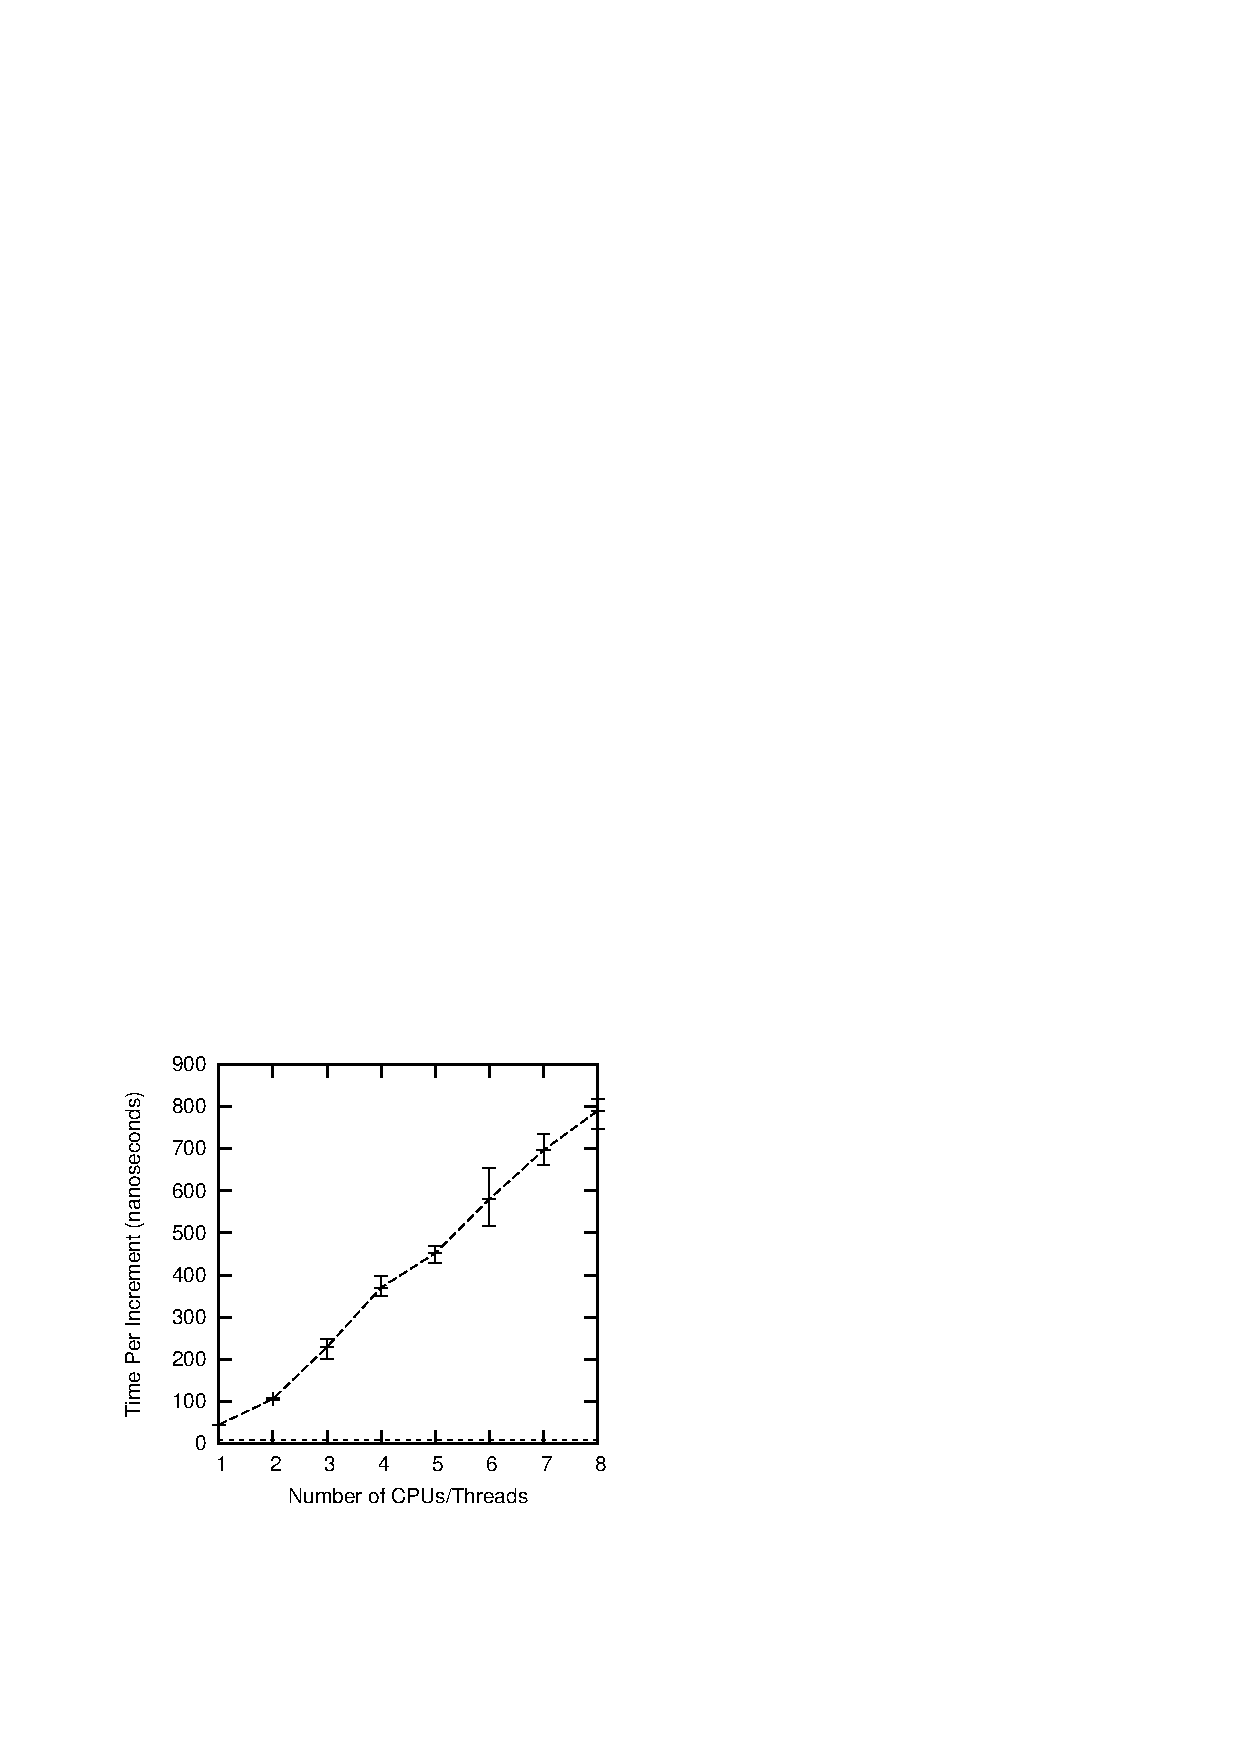
\includegraphics{CodeSamples/count/atomic}}
\end{center}
\caption{Atomic Increment Scalability}
\label{fig:count:Atomic Increment Scalability}
\end{figure}

The straightforward way to count accurately is to use atomic operations,
as shown in
Figure~\ref{fig:count:Just Count Atomically!}.
Line~1 defines an atomic variable, line~5 atomically increments it, and
line~10 reads it out.
Because this is atomic, it keeps perfect count.
However, it is slower: on a Intel Core Duo laptop, it is about
six times slower than non-atomic increment
when a single thread is incrementing, and more than \emph{ten times}
slower if two threads are incrementing.
This should not be a surprise, given the discussion in
Chapter~\ref{chp:Hardware and its Habits},
nor should it be a surprise that the performance of atomic increment
gets slower as the number of CPUs and threads increase, as shown in
Figure~\ref{fig:count:Atomic Increment Scalability}.
The additional CPUs and threads must simply wait in line for
access to the counter.

@@@ diagrams and explanation @@@

\QuickQuiz{}
	But atomic increment is still pretty fast.
	And incrementing a single variable in a tight loop sounds
	pretty unrealistic to me, after all, most of the program's
	execution should be devoted to actually doing work, not accounting
	for the work it has done!
	Why should I care about making this go faster?
\QuickQuizAnswer{
	In many cases, atomic increment will in fact be fast enough
	for you.
	In those cases, you should by all means use atomic increment.
	That said, there are many real-world situations where
	more elaborate counting algorithms are required.
	The canonical example of such a situation is counting packets
	and bytes in highly optimized networking stacks, where it is
	all too easy to find much of the execution time going into
	these sorts of accounting tasks, especially on large
	multiprocessors.

	In addition, counting provides an excellent view of the
	issues encountered in shared-memory parallel programs.
} \QuickQuizEnd

The following sections discuss high-performance counting.

\section{Statistical Counters}
\label{sec:count:Statistical Counters}

Split counters.

\QuickQuiz{}
	What fundamental difference is there between counting packets
	and counting the total number of bytes in the packets, given
	that the packets vary in size?
\QuickQuizAnswer{
	When counting packets, the counter is only incremented by the
	value one.
	On the other hand, when counting bytes, the counter might
	be incremented by largish numbers.

	Why does this matter?
	Because in the increment-by-one case, the value returned will
	be exact in the sense that the counter must necessarily have
	taken on that value at some point in time, even if it is impossible
	to say exactly when that point occurred.
	In contrast, when counting bytes, two different threads might
	return values that are inconsistent with any global ordering
	of operations.

	To see this, suppose that thread~0 adds the value three to its
	counter, thread~1 adds the value five to its counter, and
	threads~2 and 3 sum the counters.
	If the system is ``weakly ordered'' or if the compiler
	uses aggressive optimizations, thread~2 might find the
	sum to be three and thread~3 might find the sum to be five.
	The only possible global orders of the sequence of values
	of the counter are 0,3,8 and 0,5,8, and neither order is
	consistent with the results obtained.

	If you missed this one, do not feel bad.
	Michael Scott used this question to stump Paul McKenney during Paul's
	Ph.D. defense.
} \QuickQuizEnd


\section{Read-At-End Counters}
\label{sec:count:Read-At-End Counters}

reduce phase of map-reduce.

\section{Atomic-Read Reference Counters}
\label{sec:count:Atomic-Read Reference Counters}

\section{Limit Counters}
\label{sec:count:Limit Counters}

\section{Double-Limit Counters}
\label{sec:count:Double-Limit Counters}

\section{Discussion}
\label{sec:count:Discussion}

This chapter has presented the reliability, performance, and
scalability problems with traditional counting primitives.
The C-language \url{++} operator is not guaranteed to function reliably in
multithreaded code, and atomic operations to a single variable neither
perform nor scale well.
This chapter has also presented a number of counting algorithms that
perform and scale extremely well in certain special cases.

The fact that these algorithms only work well in their respective special
cases might be considered a major problem with parallel programming in
general.
After all, the C-language \url{++} operator works just fine in single-threaded
code, and not just for special cases, but in general, right?

This line of reasoning does contain a grain of truth, but is in essence
misguided.
The problem is not parallelism as such, but rather scalability.
To understand this, first consider the C-language \url{++} operator.
The fact is that it does \emph{not} work in general, only for a restricted
range of numbers.
If you need to deal with 1,000-digit decimal numbers, the C-language \url{++}
operator will not work for you.

\QuickQuiz{}
	The \url{++} operator works just fine for 1,000-digit numbers!!!
	Haven't you heard of operator overloading???
\QuickQuizAnswer{
	In the C++ language, you might well be able to use \url{++}
	on a 1,000-digit number, assuming that you had access to a
	class implementing such numbers.
	But as of 2009, the C language does not permit operator overloading.
} \QuickQuizEnd

This problem is not specific to arithmetic.
Suppose you need to store and query data.
Should you use an ASCII file, XML, a relational database, a linked list,
a dense array, a B-tree, a radix tree, or any of the plethora of other data
structures and environments that permit data to be stored and queried?
It depends on what you need to do, how fast you need it done, and how
large your data set is.

Similarly, if you need to count, your solution will depend on how large
of numbers you need to work with, how many CPUs need to be manipulating
a given number concurrently, how the number is to be used, and what
level of performance and scalability you will need.

Nor is this problem specific to software.
The design for a bridge meant to allow people to walk across a small brook
might be a simple as a plank thrown across the brook.
But this solution of using a plank does not scale.
You would probably not use a plank to span the kilometers-wide mouth of
the Columbia River, nor would such a design be advisable for bridges
carrying concrete trucks.

In short, just as bridge design has changed as their spans and loads have
increased, so will software design change as the number of CPUs increases.
An important tool permitting large numbers of CPUs to be brought to bear
is \emph{partitioning}, which will be considered in greater depth in the
next chapter.
